\chapter{Perancangan}
\label{chap:perancangan}

\section{Struktur Penyimpanan Leksikon}
\label{sec:strukturPenyimpananLeksikon}

Leksikon yang dirancang pada perangkat lunak morphological parser ini akan menyimpan kata dasar dan kata turunan yang valid dalam bahasa Indonesia. Kata dasar secara khusus akan dimuat ke dalam program dalam sebuah struktur data trie supaya dapat diakses dengan cepat dan efektif. Sementara kata turunan akan diakses setelah proses parsing selesai untuk melakukan validasi terhadap hasil dari proses parsing. Kata dasar dan kata turunan tersebut harus disimpan dalam file khusus supaya dapat dimuat dan diakses oleh program ketika program dijalankan.

Semua kata dasar disimpan pada sebuah file yang bernama 'roots' berekstensi '.lxc' pada sebuah folder dalam program. Setiap entri kata dasar dipisahkan oleh karakter enter dan disimpan terurut berdasarkan urutan abjad. Untuk menyimpan kata turunan dari setiap kata dasar, dibuat sebuah file khusus dengan nama file sama dengan kata dasar dan berekstensi '.lxc' yang disimpan pada folder yang sama. Isi dari setiap file tersebut adalah kata dasar diikuti oleh semua kemungkinan kata turunan yang dapat dibentuk dari kata dasar yang bersangkutan.

Penyimpanan kata turunan tidak bisa dilakukan dengan menulis semua bentuk turunan secara langsung karena akan sangat tidak efisien, terutama untuk bentuk turunan dari afiks yang sangat produktif seperti prefiks \textit{ber-} dan prefiks \textit{me-}. Perlu struktur khusus untuk menyimpan semua kata turunan dengan efisien dalam setiap file kata dasar. Oleh karena itu, dirancang beberapa lambang leksikon seperti dapat dilihat pada tabel \ref{tabel-lambang-leksikon} berikut.

\begin{table}[H]
\centering
\begin{tabular}{|c|c|}
\hline
\textbf{Bentuk} & \textbf{Lambang leksikon} \\
\hline
Komposisi&@\\
Reduplikasi&\textasciicircum\\
Prefiks&[\\
Sufiks&]\\
Konfiks&\# ..-..\\
\hline
\end{tabular}
\caption{Tabel Lambang Bentuk Turunan dalam Leksikon} 
\label{tabel-lambang-leksikon}
\end{table}

Untuk menyimpan kata turunan 'sayur bening' yang merupakan hasil proses komposisi dari kata 'sayur' digabung dengan kata 'bening', kita bisa menambahkan bentuk '@bening' dalam file 'sayur.lxc'. Untuk menyimpan kata 'sayur-mayur' yang merupakan hasil reduplikasi berubah bunyi dari kata 'sayur', kita bisa menuliskan bentuk '\textasciicircum mayur'. Sementara untuk bentuk turunan hasil dari proses prefiksasi dan sufiksasi seperti kata 'menyayur' dan 'sayuran', dapat disimpan dalam bentuk '[me' dan ']an'. Untuk kata yang merupakan hasil dari proses konfiksasi seperti kata 'kesatuan', kita bisa menyimpannya dalam file 'satu.lxc' dengan bentuk '\# ke-an'.

Suatu kata turunan dapat dibentuk dari lebih dari satu proses morfologi, misalnya kata 'sayur-sayuran' yang merupakan kata dasar 'sayur' yang dilakukan reduplikasi utuh menjadi 'sayur-sayur' lalu dibubuhkan sufiks \textit{-an} menjadi bentuk 'sayur-sayuran'. Untuk menyimpan bentuk tersebut, setiap proses dapat dipisahkan dengan simbol '+' dengan proses yang lebih dulu dikerjakan ditulis lebih dahulu. Untuk menyimpan bentuk reduplikasi utuh, kita bisa menyimpannya dengan bentuk '\textasciicircum 2'. Kata turunan 'sayur-sayuran' disimpan dalam file 'sayur.lxc' dengan bentuk '\textasciicircum 2+]an'.

Gambar \ref{contoh-entri-sayur} berikut adalah contoh isi dari file 'sayur.lxc' yang berisi semua kata turunan dari kata dasar 'sayur'.

\begin{figure}[H]
\centering
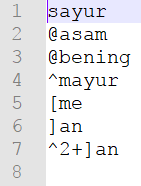
\includegraphics[scale=1]{Gambar/contoh-entri-sayur}
\caption{Isi dari file sayur.lxc} 
\label{contoh-entri-sayur}
\end{figure}

Pada kasus di mana terdapat lebih dari satu prefiks seperti pada kata 'memperkuat', maka prefiks yang lebih dulu dibubuhkan pada kata dasar ditulis terlebih dahulu. Kata 'memperkuat' disimpan dalam file 'kuat.lxc' dengan bentuk '[per+[me'. Sementara untuk kasus pada proses klofiksasi, di mana ada prefiks dan sufiks yang diimbuhkan tetapi pengimbuhannya tidak sekaligus, urutan penulisannya adalah sufiks ditulis lebih dahulu dari prefiks. Contohnya pada kata 'berlarian' disimpan dalam file 'lari.lxc' dalam bentuk ']an+[ber'.


\section{Syntax Keluaran Proses Morphological Parsing}
\label{sec:syntaxKeluaran}

\section{Perancangan Antarmuka}
\label{sec:perancanganAntarmuka}

\section{Diagram Kelas Lengkap}
\label{sec:DiagramKelasLengkap}